\chapter{Desarrollo}
\label{chap:desarrollo}

\drop{C}{  omo} ya se ha comentado antes, el desarrollo de este proyecto ha supuesto un reto importante ya que las tecnologías utilizadas eran totalmente desconocidas. En este capítulo se explica el proceso seguido a lo largo de su desarrollo, además de presentar los principales problemas encontrados y las soluciones con las que se han abordado.

\section{Entrega 0}

El objetivo de esta primera entrega fue, por un lado, establecer la estructura principal del proyecto y esbozar una primera versión del a narrativa y por otro realizar una primera toma de contacto con el desarrollo de Unity, las tecnologías \acs{VR} e instalar y configurar el entorno de desarrollo para poder empezar a trabajar en la siguiente entrega.

\subsection{Estructuración del proyecto}

El primer paso lógico tras proponer al tutor de este \acs{TFM} el proyecto y ser aprobado fue empezar a definirlo. Para ello, y partiendo de la idea principal de desarrollar una experiencia de juego haciendo uso de tecnologías \acs{VR} que pusiera en contacto con el mundo del arte a personas que suelen y no visitar museos, se generó el documento que puede verse en el anexo \ref{anexo:guia-salas}. 

Este documento comienza a detallar la narrativa del juego y la integra en una visita por un museo ficticio y, aunque terminó por sufrir varios cambios importantes, sirvió para definir el punto de partida del proyecto.

A lo largo de este documento se intenta crear una historia interesante para el jugador al mismo tiempo que generar un museo ficticio pero realista y coherente en el que se pueda desarrollar dicha narrativa. Para ello, se ha seguido el orden cronológico por las épocas más importantes en la historial de arte, definiendo una sala con una historia diferente para cada una.

A la hora de elegir los cuadros que se mostrarían en las salas se intentó buscar aquellos más representativos de su época. Para ello, se contó con el asesoramiento de una historiadora del arte, que ha sido quien ha dado el visto bueno al rigor artístico del museo y sus salas.

\subsection{Configuración del entorno de desarrollo}

Antes de poder empezar a desarrollar el proyecto fue necesario elegir un \acs{IDE} y un framework con el que trabajar. Como ya se ha explicado en los capítulos \ref{chap:estado_arte} y \ref{chap:tecnologia}, tras comparar las ventajas y desventajas de los entornos de desarrollo y librerías disponibles en el mercado se decidió trabajar con Unity, el framework \acs{VRTK} y la librería SteamVR para lo que, tras instalarlas, hubo que importarlas manualmente al proyecto de Unity.

\subsection{Primera toma de contacto con Unity}

A continuación se presenta un resumen de la interfaz de Unity par que el lector pueda entender algunos de los conceptos de los que se hablará más adelante.

\begin{figure}[!h]
\begin{center}
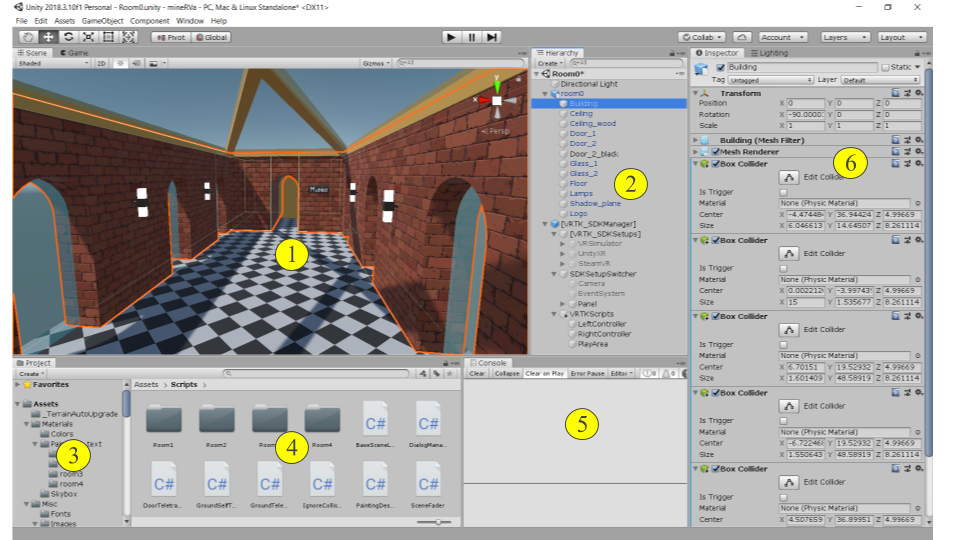
\includegraphics[width=1\textwidth]{imagenes/7/interfaz-unity.png}
\caption{Resumen de la interfaz de Unity}
\label{fig:interfaz-unity}
\end{center}
\end{figure}

\begin{enumerate}
    \item Vista de la escena actual, en la que el usuario puede obtener una vista previa de la escena e interactuar con los objetos tridimensionales para colocarlos. Funciona de manera parecida a Blender.
    
    \item Vista de la jerarquía de la escena, en la que pueden verse los objetos que hay y sus relaciones; por ejemplo, si están emparentados.
    
    \item Vista del inspector en la que aparece la información, los materiales y los componentes de un objeto seleccionado. Un componente puede ser prácticamente cualquier cosa, como un script.
    
    \item Vista del proyecto, donde aparecen todas las carpetas disponibles.
    
    \item Vista donde aparecen los elementos de la carpeta seleccionada. En este caso, pueden verse algunos de los scripts con los que se ha trabajado.
    
    \item Consola de salida en la que aparece información del proyecto.
\end{enumerate}

\section{Entrega 1}

Como se indicó en el capítulo \ref{chap:plan_entregas}, el objetivo final de las iteraciones de esta entrega fue aprender a importar modelos a Unity desde Blender y diseñar e implementar el tutorial del proyecto y que éste fuera completamente funcional. 

\subsection{Modelado e importación}

Lo primero que se hizo antes de comenzar a modelar en Blender, ya que es mucho menos productivo empezar a trabajar sin una idea previa, fue diseñar un boceto en papel en el poder basar el modelado posterior.

Como se consideró que el museo sería más realista si en lugar de empezar directamente en él el jugador tuviera que recorrer un pequeño pasillo que funcionara de antesala y desde el que se pudiera ver el exterior, fue el primer boceto que se hizo, y tras él se dibujó la sala que actuaría de tutorial. Esta sala tendría que presentar un cuadro muy reconocible y una pequeña prueba relacionada con él, por lo que se decidió utilizar el cuadro \textit{El Hijo del Hombre} de René Magritte (1964) y que el jugador tuviera que cambiar de sitio una pieza de fruta relacionada con este cuadro, de este modo aprendiendo que puede interaccionar con los elementos virtuales y que habrá relación entre las pruebas y las obras de arte de tal manera que el reto sea darse cuenta de estas ideas y no la prueba en sí. La imagen \ref{fig:bocetos-salas-0-1} muestra el boceto de estas dos salas, que fue dibujado antes de comenzar a modelarlas.

\begin{figure}[!h]
\begin{center}
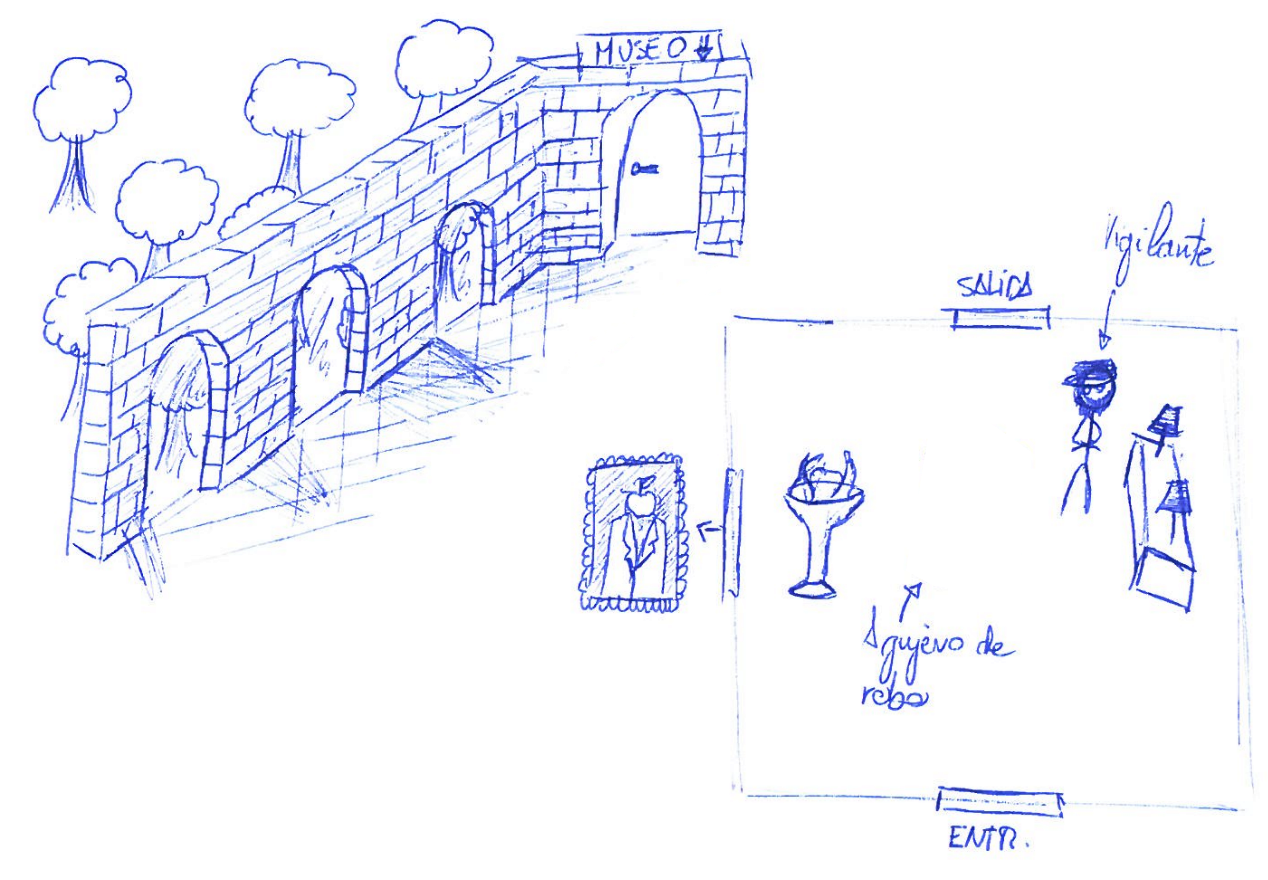
\includegraphics[width=.8\textwidth]{imagenes/7/bocetos/boceto-sala-0-1.png}
\caption{Boceto de la antesala y la sala de tutorial}
\label{fig:bocetos-salas-0-1}
\end{center}
\end{figure}

Una vez terminados los bocetos, se modeló la primera sala en Blender se comenzó a trabajar en importarla desde Unity, para lo que es necesario crear una Escena e importar en ella el archivo Blender desde el gestor de archivos. Una vez que lo hagamos, aparecerá como un \textbf{Prefab}\footnote{\url{https://docs.unity3d.com/es/current/Manual/Prefabs.html}}. De este modo, cuando el archivo Blender se modifique Unity lo detectará y actualizará su copia local, aunque por ser un Prefab no pueden modificarse desde Unity sin perder esta propiedad.

Actualmente, Blender cuenta con dos motores de renderizado; Blender Internal y Blender Cycles, y no son compatibles entre sí. Esto quiere decir que si por ejemplo creamos un material en Blender Internal y luego cambiamos a Cycles, éste no aparecerá. Aunque en teoría Unity trabaja mejor con los materiales de Blender Internal, al importarlos no aparecen como deberían y no pueden modificarse sus propiedades como su color, su \textit{metalicidad} o su mapa de normales, por lo que ha sido necesario rehacer todos los materiales de los modelos y volver a aplicarlos a mano.

Vamos a tomar como ejemplo una de las paredes de ladrillos para ver el flujo de trabajo de los materiales; tras modelarla, habría que descargar una textura para ella, para lo que se ha utilizado el sitio web \url{https://3dtextures.me/} que proporciona texturas procedurales gratuitas y con mapas de normales y rugosidad con licencia libre. Una vez hecho, se crea un material en Blender al que se le aplica la textura para ver cómo quedaría, aunque Blender Internal no da la opción de añadir más mapas a la textura. Tras esto, se importa el modelo a Unity y se crea un nuevo material, con la misma textura, al que se le añaden y configuran el resto de mapas.

La imagen \ref{fig:unity-sala-0} muestra el resultado final del modelado y la importación a Unity. Como el exterior con árboles, que puede verse a través de las ventanas, se reutiliza en otras salas se ha movido a una escena aparte que se importa cuando es necesario, recudiendo de este modo el peso de los modelos.

\begin{figure}[!h]
\begin{center}
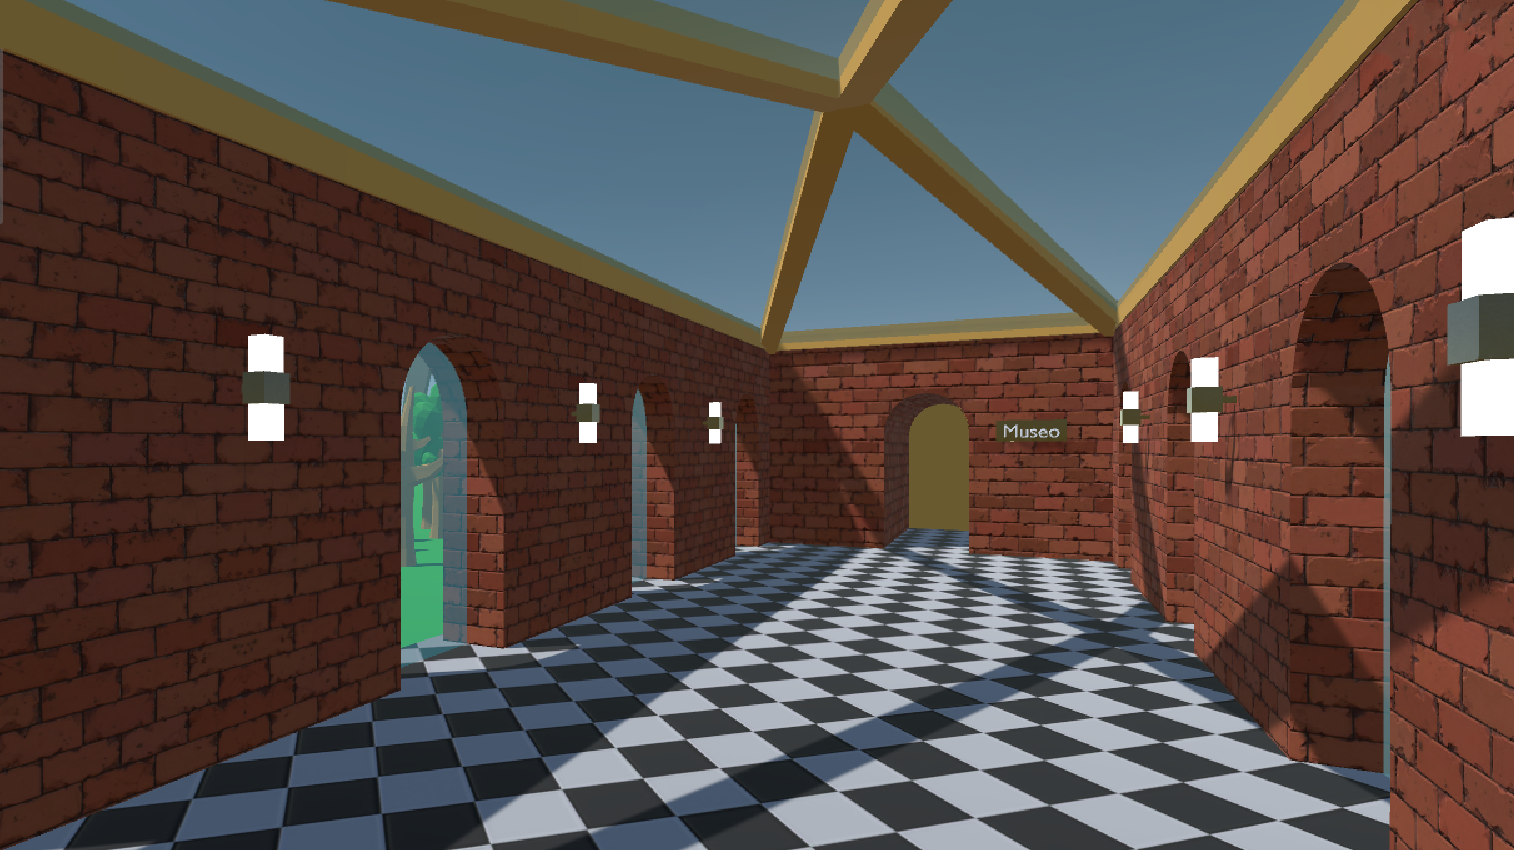
\includegraphics[width=0.85\textwidth]{imagenes/7/salas-unity/unity-sala-0.png}
\caption{Sala 0 vista desde Unity}
\label{fig:unity-sala-0}
\end{center}
\end{figure}

Tras ello se hizo lo mismo con la sala de tutorial, que puede verse en la figura \ref{fig:unity-sala-1}.

\begin{figure}[!h]
\begin{center}
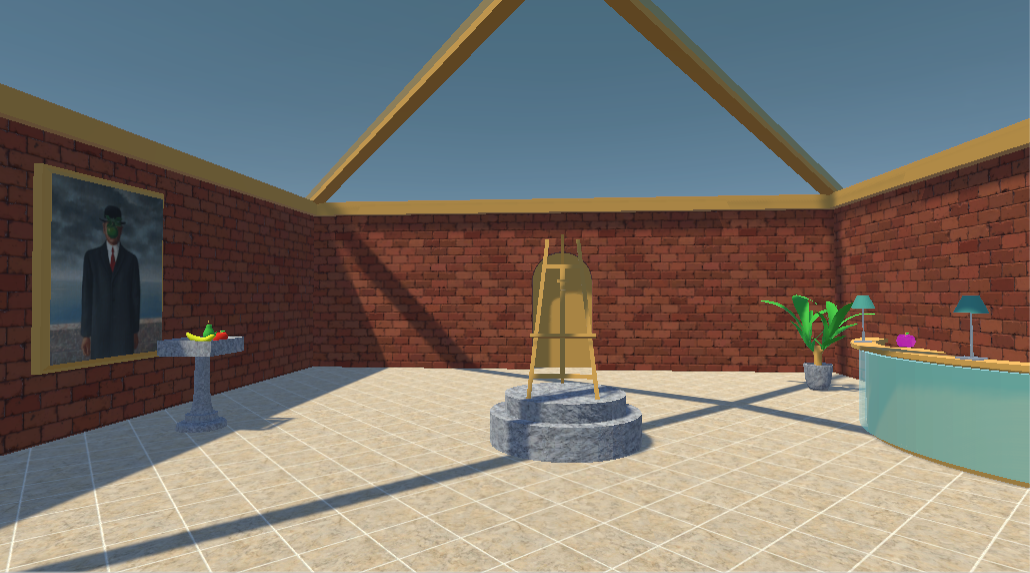
\includegraphics[width=0.85\textwidth]{imagenes/7/salas-unity/unity-sala-1.png}
\caption{Sala 1 vista desde Unity}
\label{fig:unity-sala-1}
\end{center}
\end{figure}

Además, aunque las cajas de colisiones automáticas de Unity funcionan bien para objetos no lo hacen para habitaciones, ya que estas cajas la rodean y no permiten detectar colisiones, por lo que ha sido necesario definir manualmente estas colisiones, para lo que se han utilizado los componentes \texttt{Box Collider} para cada una de la paredes, el techo y el suelo.

\subsection{Viajar entre salas}

Una vez que las dos salas estaban modeladas se trabajó en hacer que el jugador pudiera viajar entre ellas; por lo que se escribió un script en C\# que permitía viajar al jugador a otra sala al tocar una puerta, 

Para ello, lo primero que se hizo fue añadir una caja de colisiones a la puerta y activar la opción \texttt{Is trigger}, lo que le añade un \textit{listener} para poder activar otras funciones cuando detecte colisiones. Tras ello, se le añadió un componente tipo script, que puede verse simplificado en el listado \ref{lst:viajar-salas} que usa la clase \texttt{SceneManager} para cambiar la escena cuando el jugador colisiona con ella1. En él se declaran dos variables públicas para poder definirlas desde el propio inspector de Unity más cómodamente, como puede verse en la figura \ref{fig:door-teleporter-inspector}, lo que añade flexibilidad y realización al código.

\begin{lstlisting}[caption=Fragmento del script para viajar entre salas, label=lst:viajar-salas]
public string scene_name;
public float fadingTime = 10.0f;
public bool IsExitDoor = false;
    
private void OnTriggerEnter(Collider other)
{
    if (scene_name != "" && !SceneManager.GetSceneByName(scene_name).isLoaded)
    {
        SceneManager.LoadScene(scene_name, LoadSceneMode.Single);
    }
}
\end{lstlisting}

\begin{figure}[!h]
\begin{center}
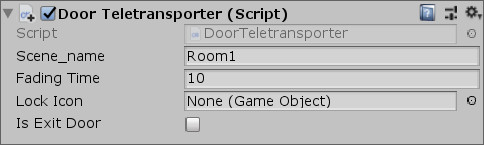
\includegraphics[width=0.6\textwidth]{imagenes/7/door-teleporter-inspector.jpg}
\caption{Script para cambiar de salas desde el inspector}
\label{fig:door-teleporter-inspector}
\end{center}
\end{figure}

Además, cada script puede implementar dos funciones, \texttt{Start()} y \texttt{Update()}, que se ejecutan automáticamente al inicio y en cada frame, respectivamente.

\subsection{Interacción con objetos virtuales}

Una vez modeladas las dos salas, se comenzó a trabajar en hacer que el jugador pudiera interactuar con los objetos virtuales. Al estar utilizando el framework \acs{VRTK} se han podido hacer uso de sus funciones para facilitar mucho el trabajo.

Lo primero que se hizo, tras modelar las tres piezas de fruta (una manzana, un plátano y una pera) fue dotarlas de físicas, para lo que se utilizaron los componentes \texttt{Box Collider} y \texttt{Rididbody}. Tras ello se hizo que interactuaran con los mandos del jugador con ayuda de los componentes \texttt{VRTK\_Interactable\_Object}, \texttt{VRTK\_Child\_Of\_Controller}, \texttt{VRTK\_Interact\_-} \texttt{Haptics} y se hizo que apareciera un borde amarillo cuando su caja de colisión detectara el mando con ayuda del componente \texttt{VRTK\_Outline\_Object\_-} \texttt{Highlighter}. Tras ello, se utilizó una \textit{snap drop zone} o zona en la que poder colocar objetos, para lo que se adaptó uno de los proporcionados por el framework.

Como resultado de esta entrega se generó el primer entregable y, por tanto, se grabó un vídeo presentando el proyecto y enseñando los avances, que puede verse en el siguiente enlace,

\begin{center}
    \url{https://youtu.be/m7rvcdZuUMI}
\end{center}


\section{Entrega 2}

\begin{figure}[!h]
\begin{center}
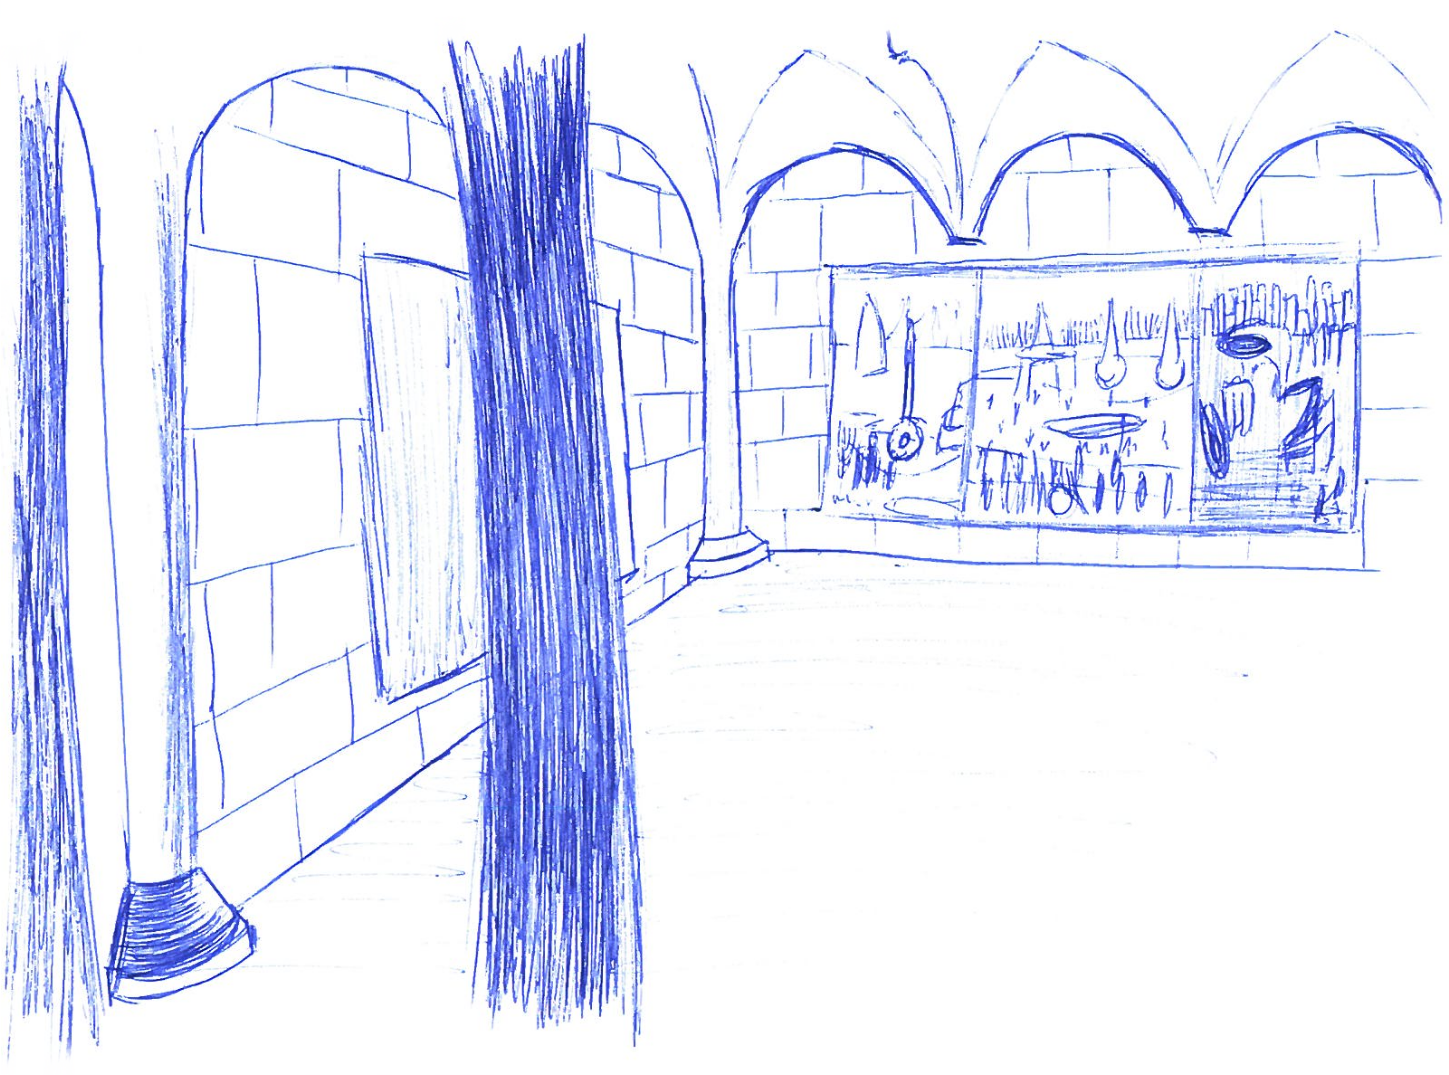
\includegraphics[width=1\textwidth]{imagenes/7/bocetos/boceto-sala-2.png}
\caption{Boceto de la segunda sala}
\label{fig:bocetos-salas-2}
\end{center}
\end{figure}

\section{Entrega 3}

\begin{figure}[!h]
\begin{center}
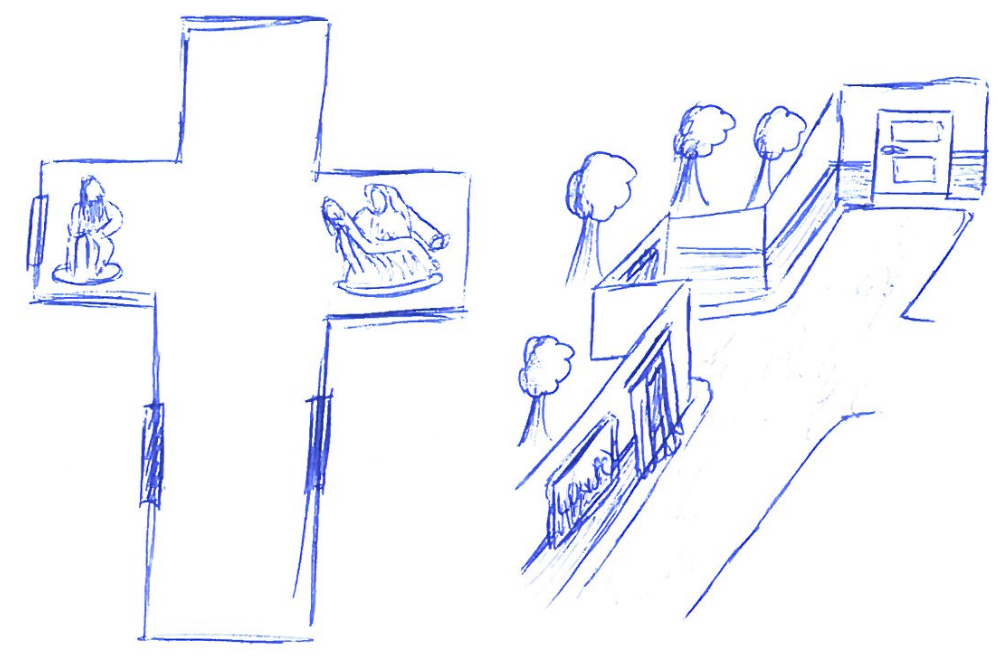
\includegraphics[width=1\textwidth]{imagenes/7/bocetos/boceto-sala-3.png}
\caption{Boceto de la tercera sala}
\label{fig:bocetos-salas-3}
\end{center}
\end{figure}

\section{Entrega 4}

\begin{figure}[!h]
\begin{center}
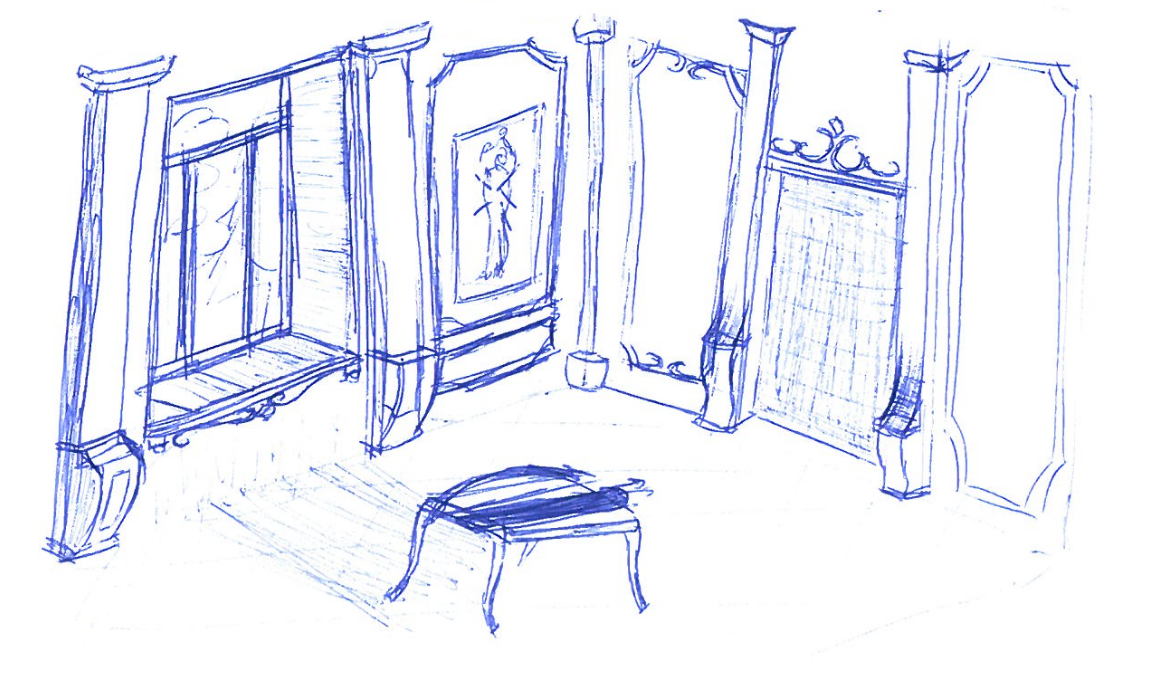
\includegraphics[width=1\textwidth]{imagenes/7/bocetos/boceto-sala-4.png}
\caption{Boceto de la cuarta sala}
\label{fig:bocetos-salas-4}
\end{center}
\end{figure}

\begin{figure}[!h]
\begin{center}
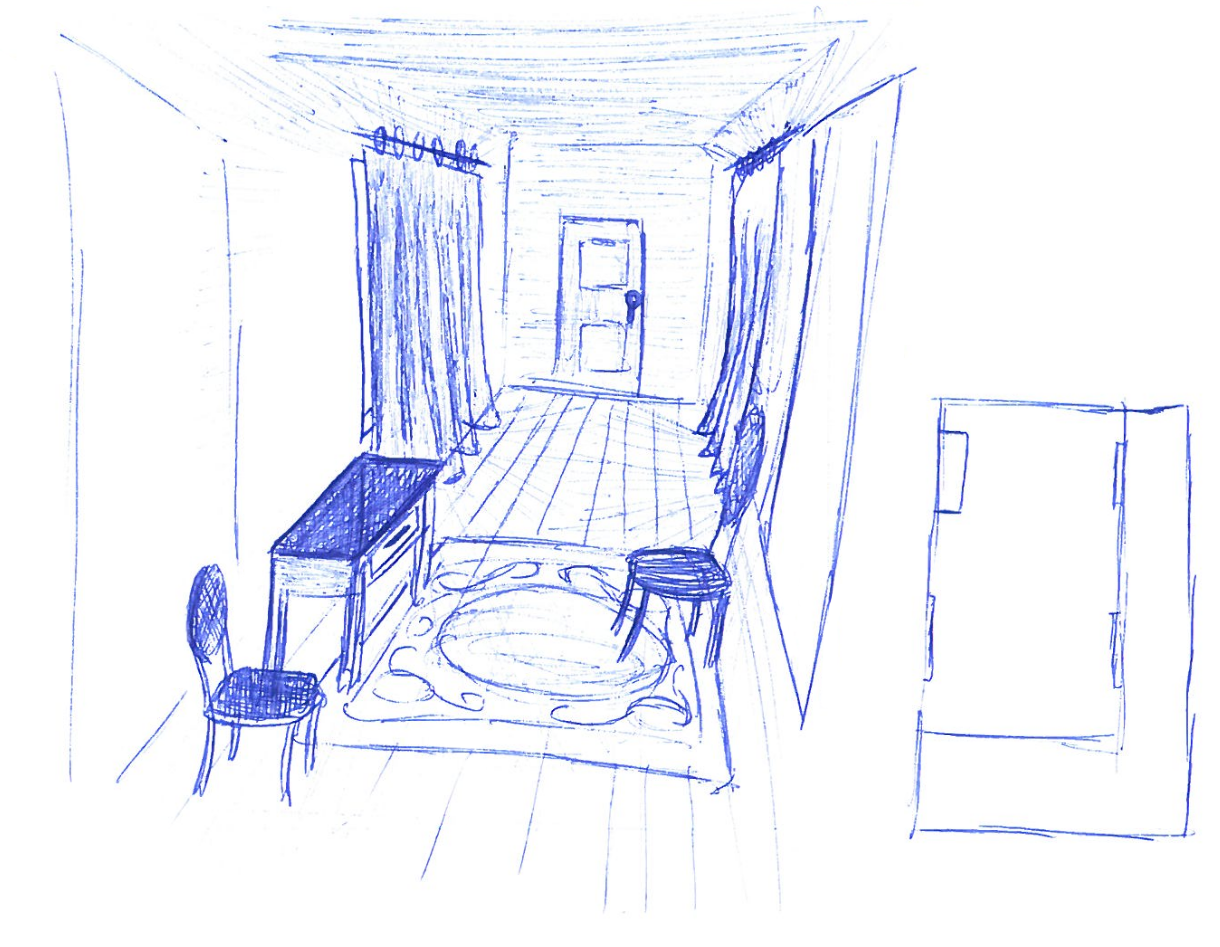
\includegraphics[width=1\textwidth]{imagenes/7/bocetos/boceto-sala-5.png}
\caption{Boceto de la quinta sala}
\label{fig:bocetos-salas-5}
\end{center}
\end{figure}

\section{Entrega 5}

\begin{figure}[!h]
\begin{center}
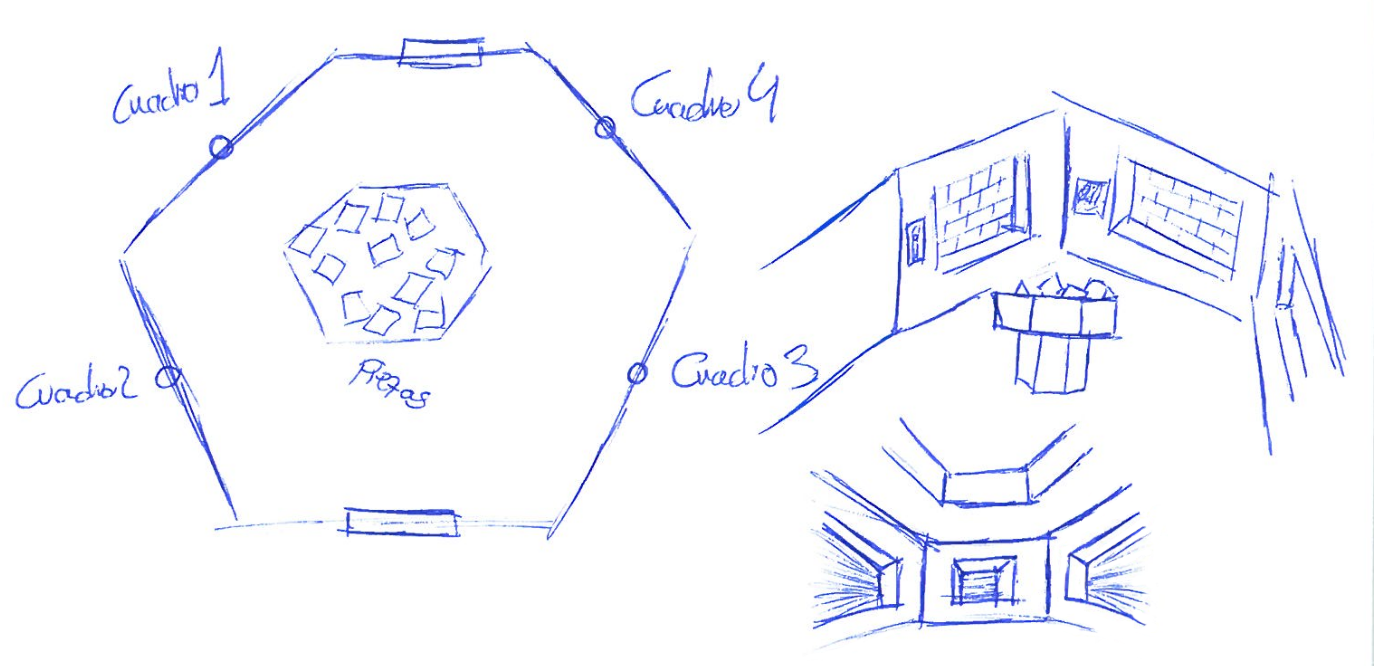
\includegraphics[width=1\textwidth]{imagenes/7/bocetos/boceto-sala-6.png}
\caption{Boceto de la sexta sala}
\label{fig:bocetos-salas-6}
\end{center}
\end{figure}

\section{Entrega 6}

